\documentclass[a4paper]{article}

\usepackage{fullpage}

\usepackage[english]{babel}
\usepackage[utf8]{inputenc}
\usepackage{amsmath}
\usepackage{graphicx}
\usepackage[colorinlistoftodos]{todonotes}
\usepackage{float}

\title{SWAGPAPER}

\author{Valle og Zach}

\date{\today}

\begin{document}
\maketitle

\section{Dataset}
Already during project 1 we noticed that the dataset could have some anomalous objects (by looking at for example a plot of the first two principal components, see figure \ref{fig_pca}). Interestingly, another version of the dataset was available, by Redmond\cite{redmond09}, which has been preprocessed in a number of ways; first each attribute has been normalized into a 0-1 interval, and then values more than 3 standard deviations above the mean are normalized to 1 while values more than 3 std. dev. below the mean are standardized to 0.

\begin{figure}[H]
\centering
  \includegraphics[width=1\linewidth]{fig_pca}
  \caption{figure}{Plot of first two principal components computed on the (standardized) raw dataset}
  \label{fig_pca}
\end{figure}

Whether we use the preprocessed dataset by \cite{redmond09} depends on what machine learning task is being performed. Unless otherwise specified, we use this preprocessed dataset.


\subsection{Association mining}
We thought it would be interesting to investigate association rules on attributes regarding race, income and violent crimes so we extracted relevant features and ran the Apriori algorithm on them.

Since our data consists mostly of ratio-attributes we had to first binarize each attribute (by setting each value to either 0 or 1 depending on whether it was above or below the median). In order to capture association rules about both low and high values, we also made duplicates of all these binarized attributes with 0 and 1 switched.

Due to the above, all item sets consisting of a single item has around 50\% support (since the values are split around the median). Therefore, we should not set minimum support for the Apriori algorithm above 50. We chose to use a minimum support of 40.

Using a minimum confidence of 80, the Apriori algorithm yields the following rules:
\begin{verbatim}
Rule: HighPctPopUnderPov <- LowmedIncome (92.0782)
Rule: HighmedIncome <- LowPctPopUnderPov (92.0455)
Rule: LowmedIncome <- HighPctPopUnderPov (87.232)
Rule: LowPctPopUnderPov <- HighmedIncome (87.182)
Rule: HighracePctWhite <- Lowracepctblack (83.299)
Rule: Highracepctblack <- LowracePctWhite (83.1601)
Rule: HighViolentCrimesPerPop <- LowracePctWhite Highracepctblack (82.125)
\end{verbatim}
Some of which are not of much interest (for example, that a community with low median income is likely to also have a high percent of population under poverty is not a big surprise). What is somewhat interesting, however, is the association rule that communities that a low percentage of white population combined with a high percentage of black population is likely to also has a high number of violent crimes per capita.

The reason we chose to extract only a few features, was that the number of found rules quickly grew out of hand when using the full dataset.



\subsection{Outlier and anomaly detection}
Since the preprocessed dataset by \cite{redmond09} already had some outlier handling done, this segment was performed on the a version of the dataset that has simply been standardized (0 mean and unit variance).

Anomaly detection was performed, by ranking objects in terms of the Gaussian Kernel density (see figure \ref{fig_anom_gauss}), K-Nearest Neighbours density (see figure \ref{fig_anom_knn}), K-Nearest Neighbours Average Relative density (see figure \ref{fig_anom_knn_avgrel}) and distance to Kth nearest neighbour for K=5 (see figure \ref{fig_anom_kndist}). When all four methods agree, there is a higher probability that the anomaly is the result of some other mechanism. We also ran the outlier scoring methods in multiple iterations, by removing the object with the worst outlier score if the ranking methods all agreed.

In order to cope with missing values, we removed any objects containing such values. We also considered using the means or medians across each attribute as replacements for the missing values, but we figured that could hide potential anomalies (for example an object with extreme values in one attribute, but missing values for others which would be set to the mean or median). 

\begin{table}[H]
\begin{tabular}{c | c c c c}
  object/method & Gaussian & KNN & KNN avg. rel. & 5th-nearest \\
  worst & 4 & 4 & 4 & 4 \\
  2nd worst & 17 & 17 & 17 & 17 \\
  3rd worst & 8 & 291 & 127 & 291 \
\end{tabular}
\caption{First iteration of anomaly ranking}
\label{table_ite1}
\end{table}

The first iteration gave the results seen in table \ref{table_ite1}. All four ranking methods agreed that object 4 ("Bemidjicity") and 17 ("Glendalecity") were the most anomalous objects. However, there is some disagreement as to the third worst object. Looking at all the graphs over outlier scores except for that of the Gaussian Kernel density estimater, we can see that the two worst objects have significantly worse scores, compared to the relative changes between the remaining 8 worst objects.

\begin{table}[H]
\begin{tabular}{c | c c c c}
  object/method
        & Gaussian
                & KNN
                        & KNN avg. rel.
                          & 5th-nearest \\
  worst     & 17  & 17  & 17  & 17   \\
  2nd worst & 8   & 291 & 127 & 291  \\
  3rd worst & 251 & 8   & 117 & 8
\end{tabular}
\caption{Second iteration of anomaly ranking (after removal of object 4)}
\label{table_ite2}
\end{table}

\begin{table}[H]
\begin{tabular}{c | c c c c}
  object/method
        & Gaussian
                & KNN
                        & KNN avg. rel.
                          & 5th-nearest \\
  worst     & 8   & 291 & 127 & 291 \\
  2nd worst & 251 & 8   & 117 & 8   \\
  3rd worst & 89  & 251 & 101 & 117 
\end{tabular}
\caption{Third iteration of anomaly ranking (after removal of object 4 and 17)}
\label{table_ite3}
\end{table}

The second and third iterations were made in order to investigate whether there would be a difference between the top worst ojects found by a single rank computation, versus iteratively ranking and removing the worst object. This was not the case, though.

In conclusion, there was agreement from all four ranking methods that objects 4 and 17 were anomalous, less agreement that object 8 was anomalous, and even lesser agreement that objects 117, 251 and 291 were anomalous. As such, it might potentially be useful to remove these anomalous objects, perhaps even during preprocessing.

On a side note, running the ranking methods on the preprocessed dataset, not even the first iteration agreed on an anomalous object, which was to be expected since outiers had already been handled in that dataset.


\begin{figure}[H]
\centering
\begin{minipage}{.45\textwidth}
  \centering
  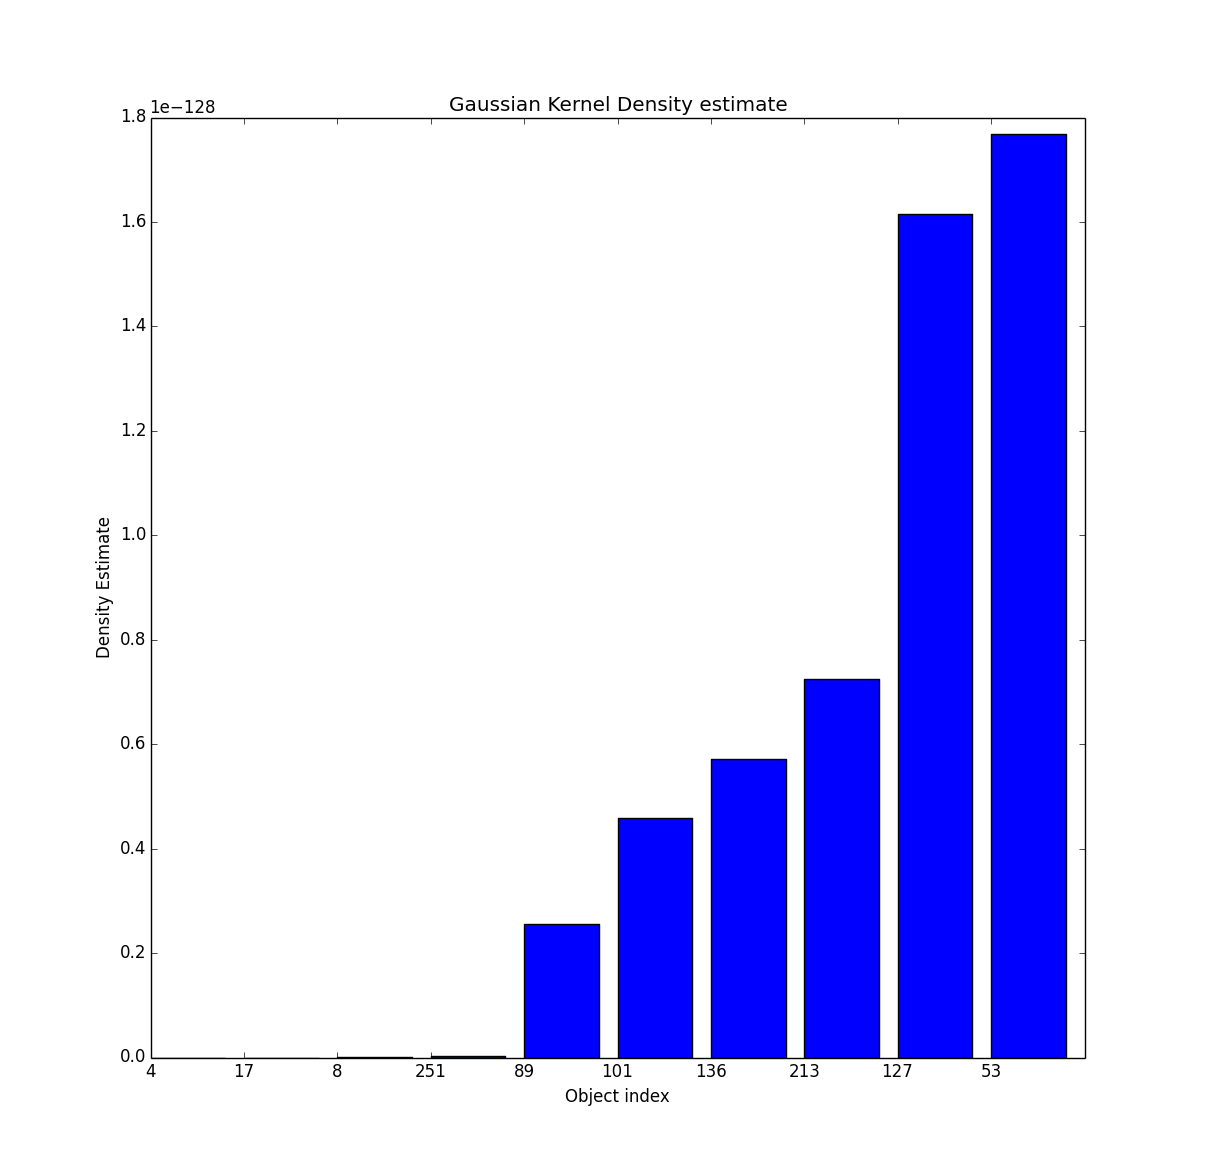
\includegraphics[width=1\linewidth]{fig_anomaly_kde_gauss}
  \caption{figure}{Plot of 10 objects with worst outlier score in terms of the Gaussian Kernel density estimater}
  \label{fig_anom_gauss}
\end{minipage}\hfill
\begin{minipage}{.45\textwidth}
  \centering
  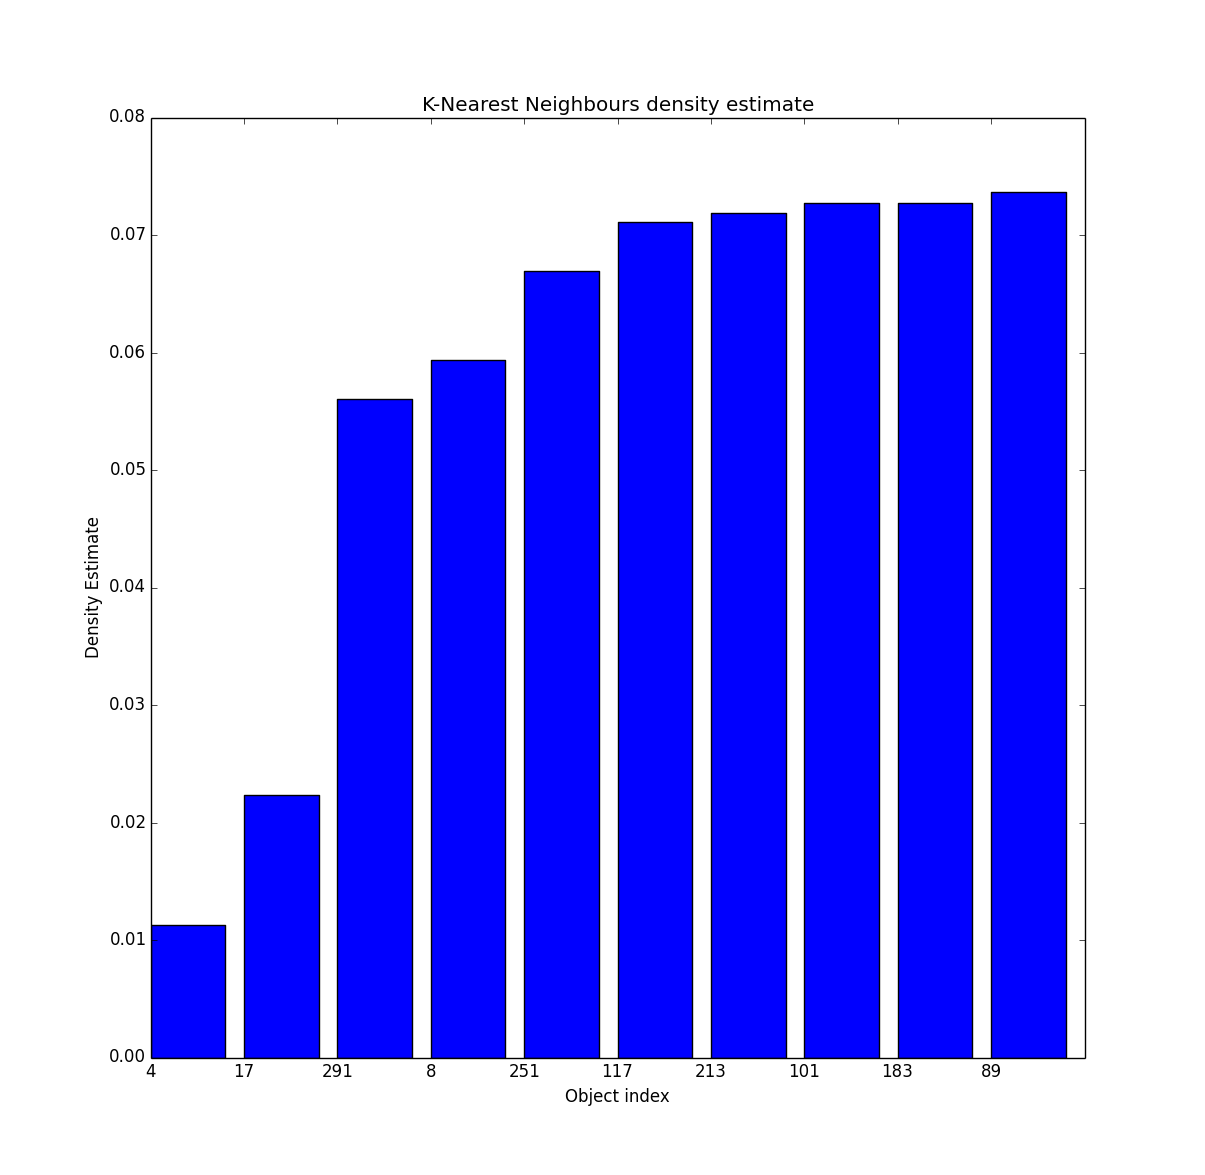
\includegraphics[width=1\linewidth]{fig_anomaly_knn_de}
  \caption{figure}{Plot of 10 objects with worst outlier score in terms of the K-Nearest Neighbours density estimater}
  \label{fig_anom_knn}
\end{minipage}
\end{figure}




\begin{figure}[H]
\centering
\begin{minipage}{.45\textwidth}
  \centering
  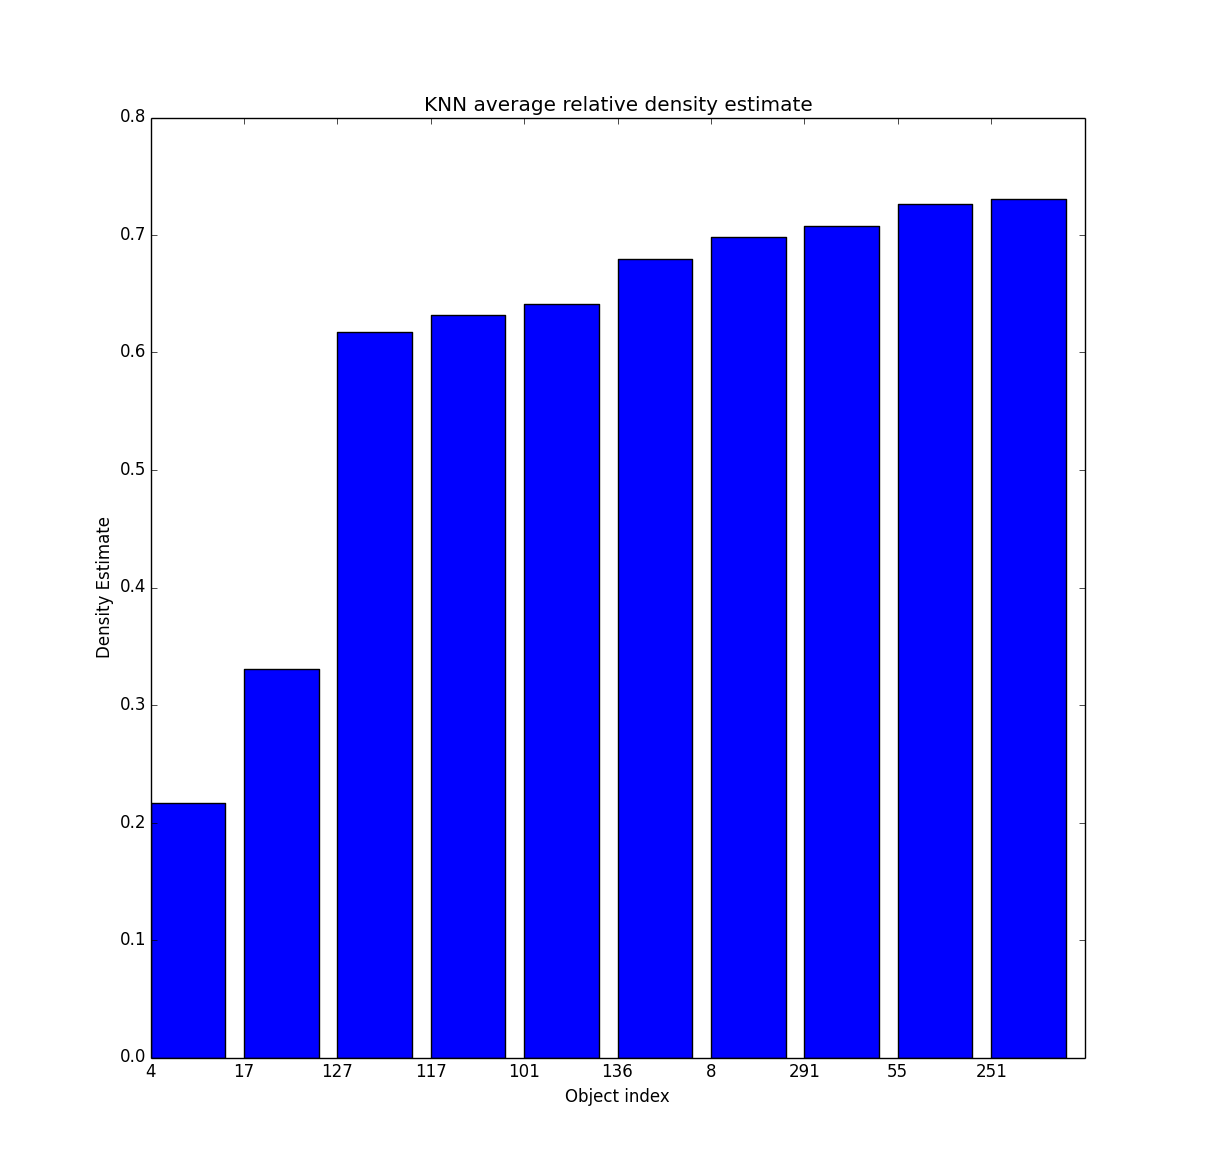
\includegraphics[width=0.9\linewidth]{fig_anomaly_knn_avgrel_de}
  \caption{Plot of 10 objects with worst outlier score in terms of the K-Nearest Neighbours average relative density estimater}
  \label{fig_anom_knn_avgrel}
\end{minipage}\hfill
\begin{minipage}{.45\textwidth}
  \centering
  \includegraphics[width=0.9\linewidth]{fig_anomaly_kndist}
  \caption{Plot of 10 objects with worst outlier score in terms of the Kth Neighbours distance}
  \label{fig_anom_kndist}
\end{minipage}
\end{figure}


\begin{thebibliography}{9}

\bibitem{redmond09}
  Michael Redmond,
  \emph{Communities and Crime}.
  Computer Science; La Salle University; Philadelphia, PA, 19141, USA,
  2009

\end{thebibliography}



\end{document}